\section{Data Extraction}
\label{sec:algorithm}
First step in the program work is to load data and to compute connected components. Data is stored in GML file format. More detail information about this format and other common graph file formats is explained in Section~\ref{sec:algorithm}.

\subsection{Dataset Description}
\label{sec:dataset_description}
Gene Ontology data and cluster analysis results presented as directed graphs. They are stored in separate files in special format -- GML files.


GO graph is directed acyclic graph has 10,042 vertices and  24,155 edges. It has 1 root, 2,729 nodes and 7,312 leafs (terminal nodes). Figure~\ref{fig:yed_GO_vis} shows visualization of the Gene Ontology graph using Hierarchical layout by yEd~\cite{yed} graph editing tool. It obviously shows imperfectness of classic visualization of the graphs.


\begin{figure}[h!]
\centering
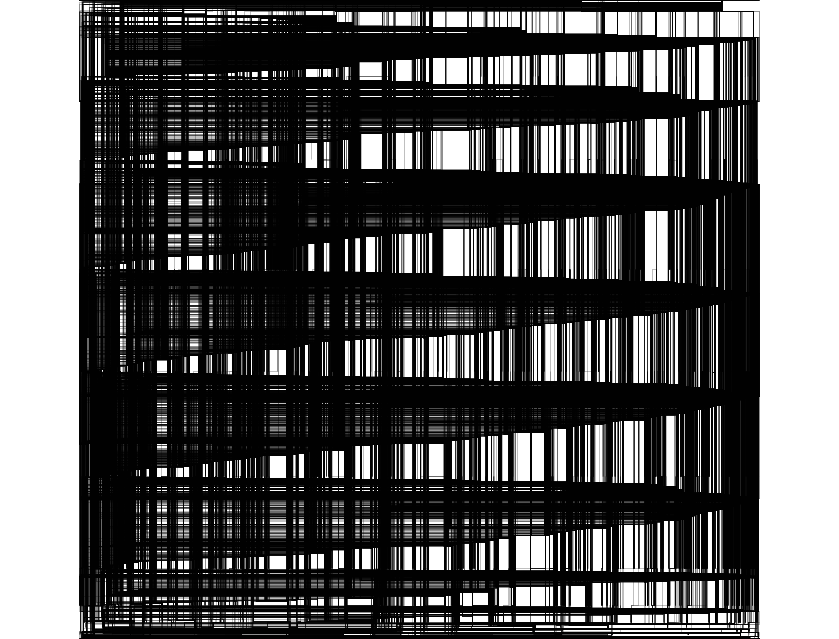
\includegraphics[scale=0.3]{pictures/yEd_GO.png}
\caption{Gene Ontology yEd visualization}
\label{fig:yed_GO_vis}
\end{figure}


Cluster graph is a directed binary tree has 14,623 nodes and 14,622 edges. The Cluster graph as a tree has a single root, 7,310 nodes and 7,312 leafs. To get an impression of the graph, Figure~\ref{fig:Cytoscape_Cluster_1} shows a cluster tree using the Cytoscape~\cite{Cytoscape} visualization tool.

\begin{figure}[h!]
\centering
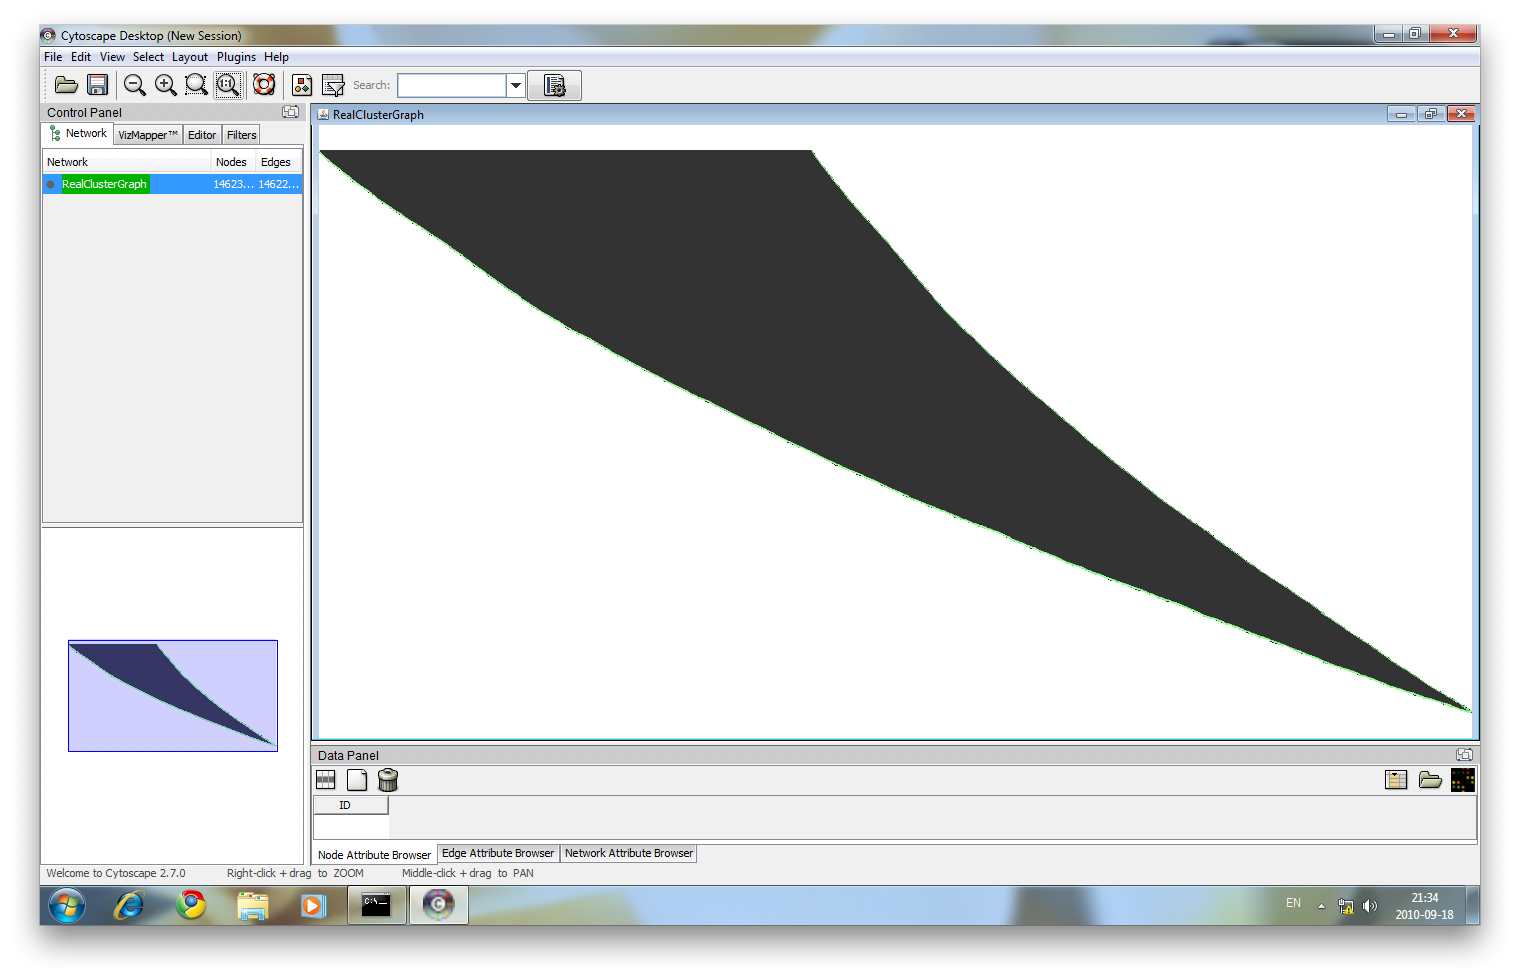
\includegraphics[scale=0.25]{pictures/Cytoscape_cluster_graph_1.png}
\caption{Cluster analysis result tree Cytoscape visualization tool}
\label{fig:Cytoscape_Cluster_1}
\end{figure}

\begin{figure}[h!]
\centering
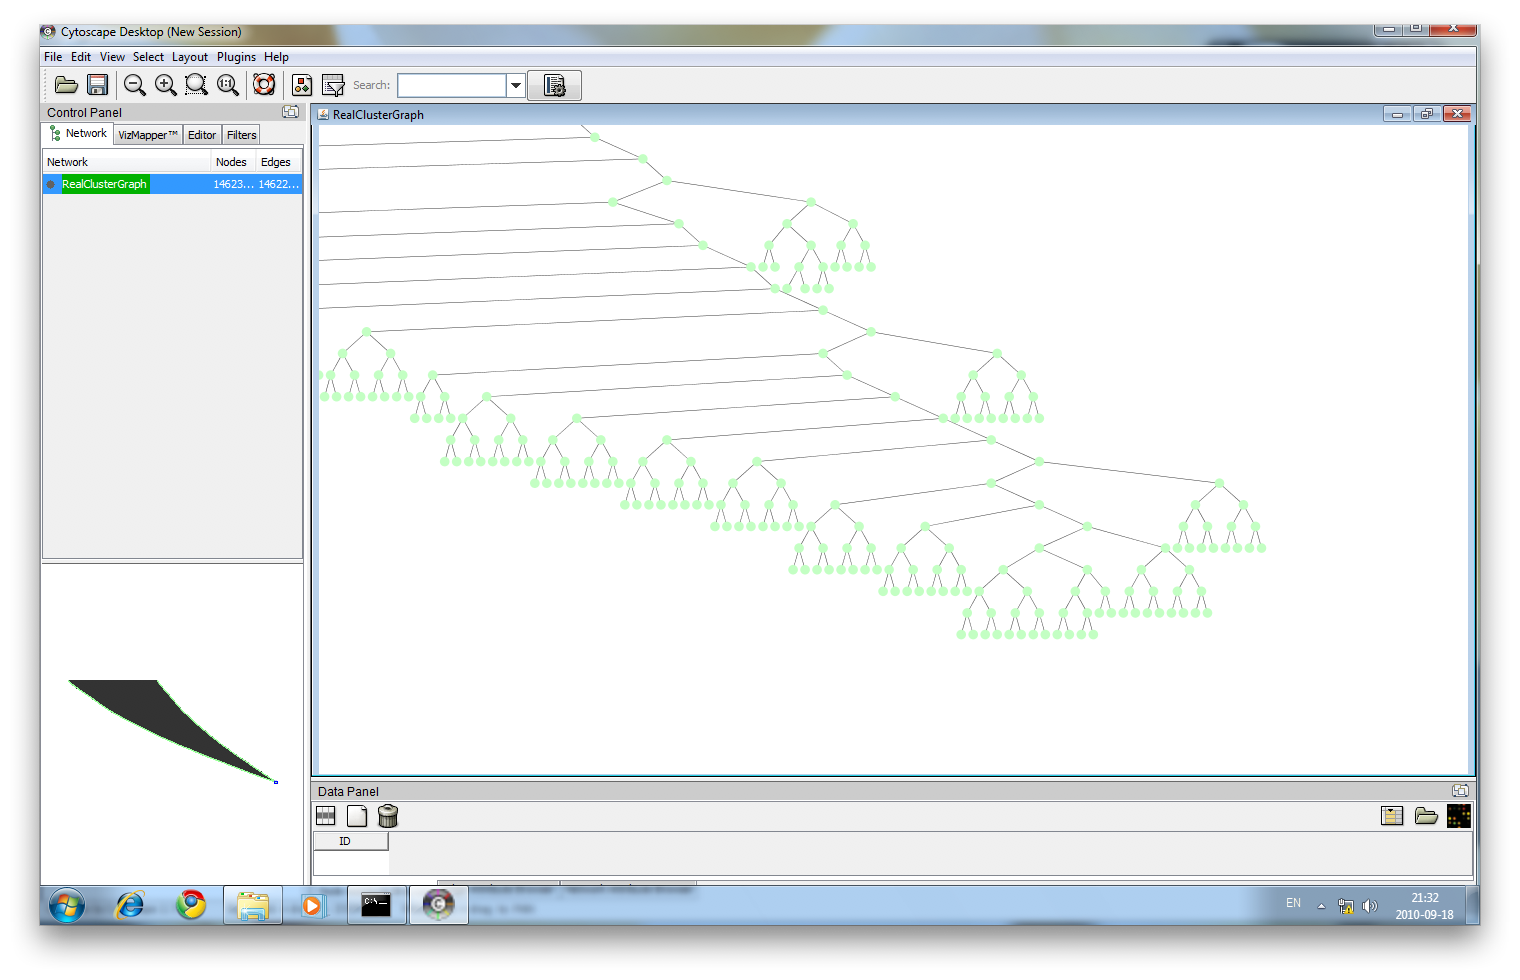
\includegraphics[scale=0.25]{pictures/Cytoscape_cluster_graph_2.png}
\caption{Zoomed cluster analysis result tree}
\label{fig:Cytoscape_Cluster_2}
\end{figure}

Both graphs are independent from each other from developer point of view: they have different node ids and edge ids. But they are corresponded by graph node labels -- both of this graphs have same label for terminal (leaf) graph nodes. This property is used in the sub-graph extracting algorithm.


The application should work with large quantity of data over tens of thousands that is why performance is one of the main requirements. It is important to give a consideration on optimization.


\subsection{Mapping Algorithm}
\label{sec:mapping_algorithm}
Here is program algorithm explanation using sample graphs:
\begin{enumerate}

\item The program visualizes Gene Ontology and cluster analysis result tree. The visualization technique is discussed in Section~\ref{sec:solution}.

\begin{figure}[h!]
\centering
\subfloat[Selected node in the Gene Ontology]{
    \label{fig:step_1}
    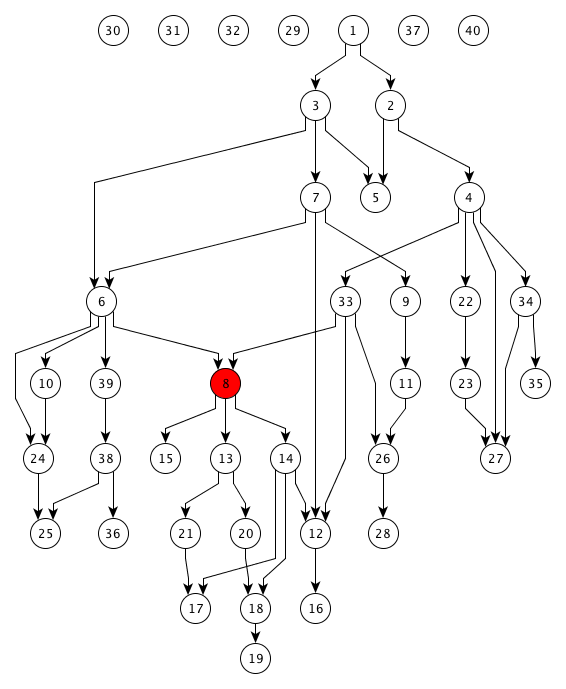
\includegraphics[scale=0.3]{pictures/subgraph_extraction_algorithm_step_1.png}
}
\subfloat[Extract sub-graph for selected node]{
    \label{fig:step_2}
    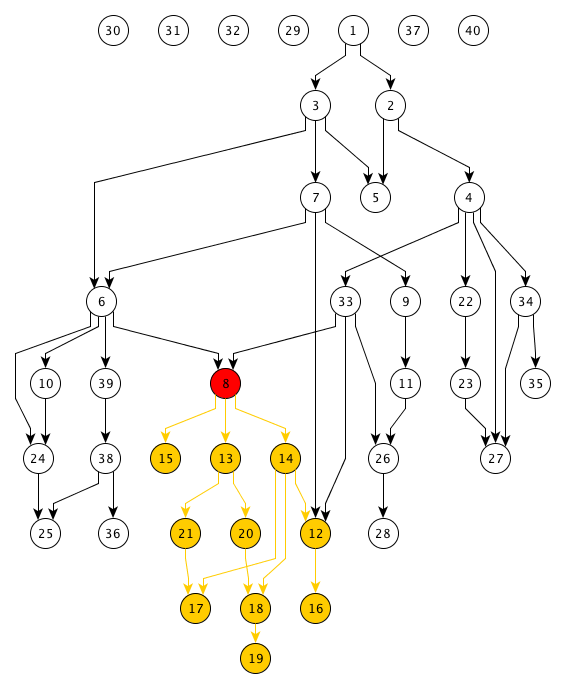
\includegraphics[scale=0.3]{pictures/subgraph_extraction_algorithm_step_2.png}
}
\caption{Sub-graph extraction from the Gene Ontology}
\end{figure}

\item Interactively select node in the Gene Ontology graph (Figure~\ref{fig:step_1}).

\item When node is selected in the Gene Ontology program computes all successors (Figure~\ref{fig:step_2}).

\item Extract leafs from successors (Figure~\ref{fig:step_3}).

\begin{figure}[h!]
\centering
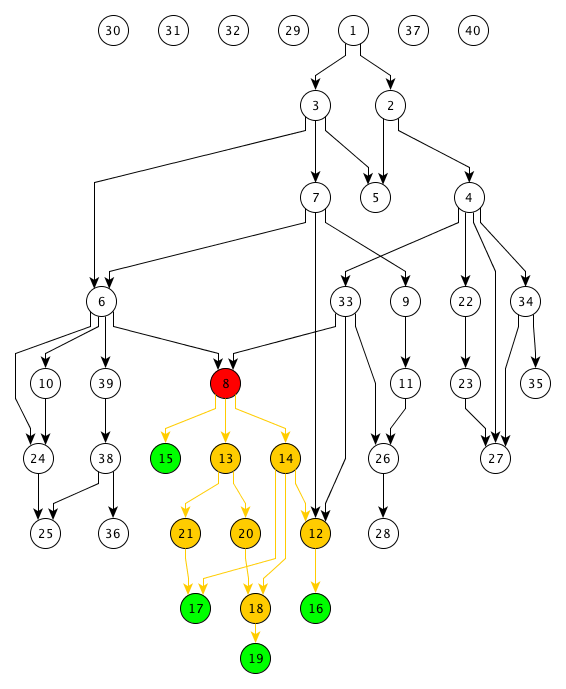
\includegraphics[scale=0.5]{pictures/subgraph_extraction_algorithm_step_3.png}
\caption{Extract leafs from the Gene Ontology sub-graph}
\label{fig:step_3}
\end{figure}

\item Founded sub tree cached. This sub tree is highlighted in cluster analysis tree.

\item Then the program searches corresponded leaves in cluster analysis result tree by label as seen in Figure~\ref{fig:step_4}.

\item For this leaves the program founds root connected to all leaves and extract corresponding sub trees (Figure~\ref{fig:step_5}).
\end{enumerate}

\begin{figure}[h!]
\centering
\subfloat[Find corresponded leafs]{
    \label{fig:step_4}
    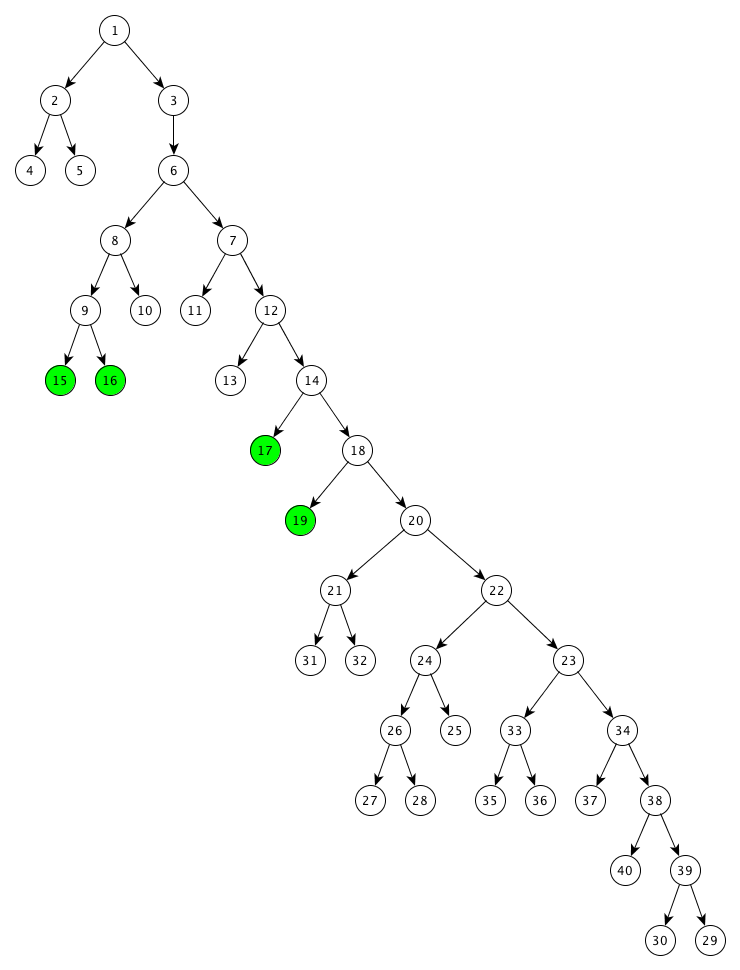
\includegraphics[scale=0.23]{pictures/subgraph_extraction_algorithm_step_4.png}
}
\subfloat[Build sub-graph]{
    \label{fig:step_5}
    
    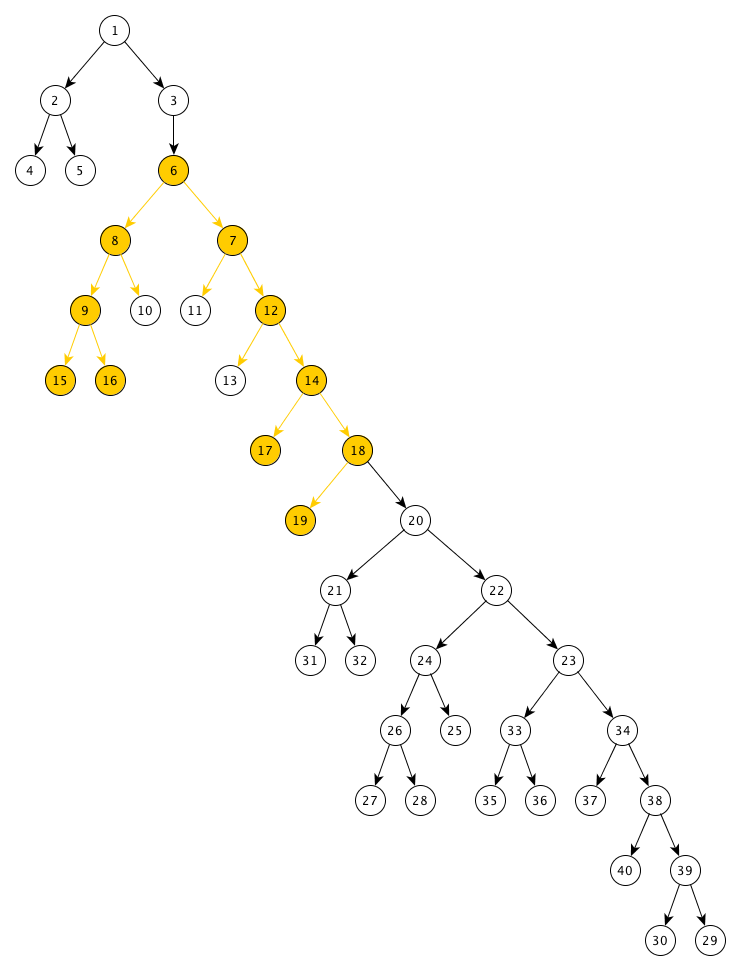
\includegraphics[scale=0.23]{pictures/subgraph_extraction_algorithm_step_5.png}
}
\caption{Analyze Cluster graph}
\end{figure}


The aim of the work is to provide flexible tool specially made for biology scientists to deal with huge data sets. Trace relations, as was discussed earlier, in the two separated datasets (Gene Ontology graph and cluster analysis result tree): both graphs are stored separately in the different files. Also during program design we should consider that cluster analysis results graph was produced from Gene Ontology graph using separate tool and clustering algorithm specific to the purpose, that means there are various cluster graphs for the same Gene Ontology.

Provide effective space filling visualization method and allow interactive relations highlighting. The tool also provides ability to track throw graphs discovering: focused or selected vertices labels for both graphs separately, Gene Ontology levels. 

Considering end-user requirements there is use case specific for biology scientist -- interest in the concrete gene in the Gene Ontology; provide search mechanism to find specific gene by name and view it.